В этом параграфе мы будем обозначать классы нулём и единицей.

Ещё один интересный метод появляется из желания посмотреть на классификацию как на задачу предсказания вероятностей.
Хороший пример -- предсказание кликов в интернете (например, в рекламе и поиске).
Наличие клика в обучающем логе не означает, что, если повторить полностью условия эксперимента, пользователь
обязательно кликнет по объекту опять.
Скорее у объектов есть какая-то \("\)кликабельность\("\), то есть истинная вероятность клика по данному объекту.
Клик на каждом обучающем примере является реализацией этой случайной величины, и мы считаем, что в пределе в каждой
точке отношение положительных и отрицательных примеров должно сходиться к этой вероятности.

Проблема состоит в том, что вероятность, по определению, величина от 0 до 1, а простого способа обучить линейную
модель так, чтобы это ограничение соблюдалось, нет.
Из этой ситуации можно выйти так: научить линейную модель правильно предсказывать какой-то объект, связанный с
вероятностью, но с диапазоном значений $(-\inf, \inf)$, и преобразовать ответы модели в вероятность.
Таким объектом является logit или log odds -- логарифм отношения вероятности положительного события к
отрицательному $\log \frac{p}{1 - p}$.

Если ответом нашей модели является $\log \frac{p}{1 - p}$, то искомую вероятность посчитать не трудно:

\begin{gather*}
(w, x\_i) = \log \frac{p}{1 - p}\\
    e^{(w, x_i)} = \frac{p}{1 - p}\\
    p = \frac{1}{1 + e^{-(w, x_i)}}\\
\end{gather*}

Таким образом, $p = \sigma ((w,x_i))$

Как теперь научиться оптимизировать $w$ так, чтобы модель как можно лучше предсказывала logit?
Нужно применить метод максимума правдоподобия для распределения Бернулли.
Это самое простое распределение, возникающее, например, при бросках монетки, которая орлом выпадает с вероятностью $p$.
У нас только событием будет не орёл, а то, что пользователь кликнул на объект с такой вероятностью.

Правдоподобие позволяет понять, насколько вероятно получить данные значения таргета $y$ при данных $X$ и весах $w$.
Оно имеет вид $p (y | X, w) = \prod_i p(y_i|x_i,w)$ и для распределения Бернулли его можно выписать так:
\[ p (y | X, w) = \prod_i p_i^{y_i}(1 - p_i)^{1 - y_i} \]
Здесь $p_i$ -- это вероятность, посчитанная из ответов модели.
Оптимизировать произведение неудобно, хочется иметь дело с суммой, так что мы перейдём к логарифмическому
правдоподобию и подставим формулу для вероятности, которую мы получили выше:
\[ l(w, X, y) = \sum_i y_i \log(p_i) + (1 - y_i) \log (1 - p_i) = \sum_i (y_i \log(\sigma ((w, x_i))) + (1 - y_i)
\log (1 - \sigma ((w, x_i)))) \]

\subsection{Базовое предположение и геометрическая интерпретация}

\underline{Вероятностная модель и предположения}

\begin{definition}[Логистическая регрессия]
    Логистическая регрессия моделирует условную вероятность принадлежности к классу 1 (бинарный случай) как:
    \[ P(y = 1 \mid \bm{x}; \bm{w}, b) = \sigma(\bm{w}^\top \bm{x} + b) = \frac{1}{1 + e^{-(\bm{w}^\top \bm{x} + b)}} \]
    Здесь $\sigma(z) = \frac{1}{1+e^{-z}}$ --- \textbf{сигмоидная (логистическая) функция}.
\end{definition}

\underline{Ключевые предположения}

\begin{enumerate}
    \item \textbf{Вероятностная модель:} предполагается, что $y_i \mid \bm{x}_i$ следуют распределению Бернулли:
    \[ y_i \mid \bm{x}_i \sim \text{Bernoulli}(p_i), \quad p_i = \sigma(\bm{w}^\top \bm{x}_i + b) \]
    
    \item \textbf{Линейность по logit (log-odds):} основное предположение --- линейная зависимость между признаками
    и \textbf{logit} вероятности:
    \[ \text{logit}(p_i) = \ln\left(\frac{p_i}{1-p_i}\right) = \bm{w}^\top \bm{x}_i + b \]
    
    \item \textbf{Условная независимость:} наблюдения $(y_i, \bm{x}_i)$ предполагаются i.i.d.
    \item \textbf{Отсутствие мультиколлинеарности:} Столбцы матрицы признаков $\bm{X}$ должны быть линейно
    независимы (для идентифицируемости модели)
\end{enumerate}

\underline{Геометрическая интерпретация}

\underline{Преобразование линейной комбинации в вероятность}

Логистическая регрессия преобразует линейную комбинацию признаков в вероятность с помощью сигмоидной функции как на
Рисунке~\ref{fig:logreg}

\begin{figure}[h]
    \centering
    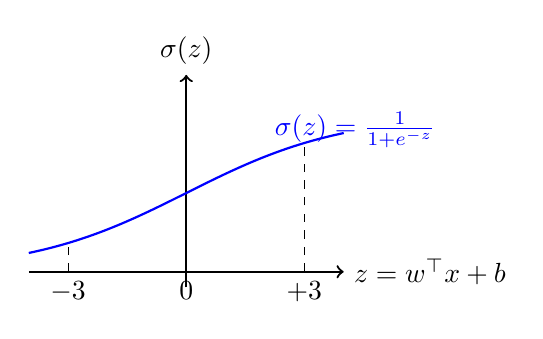
\begin{tikzpicture}[scale=1.0]
        % Первый график: линейная комбинация
        \begin{scope}[xshift=0cm]
            \draw[->, thick] (-2,0) -- (2,0) node[right] {$z = \bm{w}^\top\bm{x} + b$};
            \draw[->, thick] (0,-0.2) -- (0,2.5) node[above] {$\sigma(z)$};
            
            % Сигмоидная функция
            \draw[thick, blue] plot[smooth, domain=-2:2] (\x, {2/(1+exp(-\x))});
            
            % Вертикальные линии для интерпретации
            \draw[dashed] (-1.5,0) node[below] {$-3$} -- (-1.5,0.4);
            \draw[dashed] (0,0) node[below] {$0$} -- (0,1);
            \draw[dashed] (1.5,0) node[below] {$+3$} -- (1.5,1.6);
            
            \node[blue, right] at (1,1.8) {$\sigma(z) = \frac{1}{1+e^{-z}}$};
        \end{scope}
        
        % Второй график: разделение в пространстве признаков
%        \begin{scope}[xshift=6cm]
%            \draw[->, thick] (-1.5,0) -- (2.5,0) node[right] {$x_1$};
%            \draw[->, thick] (0,-1) -- (0,2) node[above] {$x_2$};
%
%            % Разделяющая прямая
%            \draw[thick, red] (-1,2) -- (2,0) node[midway, above left] {$\bm{w}^\top\bm{x} + b = 0$};
%
%            % Контуры вероятностей
%            \foreach i̧n {0.1,0.3,0.5,0.7,0.9} {
%                \pgfmathsetmacro{\z}{ln(\c/(1-\c))}
%                \pgfmathsetmacro{\yintercept}{-\z/0.8 + 2.5} % для w = [1, 0.8], b = -z
%                \pgfmathsetmacro{\xintercept}{\z - 2} % приблизительно
%
%                \ifdim
%                    \c pt = 0.5 pt
%                    \draw[red, thick] (-1,2) -- (2,0);
%                \else
%                    \draw[blue!50, dashed] (-0.5,\yintercept) -- (2,\xintercept);
%                \fi
%            }
%
%            % Области вероятностей
%            \node[blue!70] at (1.5,1.5) {$P(y=1) > 0.5$};
%            \node[blue!70] at (0.5,0.5) {$P(y=1) < 0.5$};
%
%            % Точки данных
%            \foreach \x/\y in {0.5/1.5, 1/1.8, 0.8/1.3, 1.5/1.5, 1.2/1.6}
%            \fill[blue] (\x,\y) circle (2pt);
%
%            \foreach \x/\y in {1/0.5, 1.5/0.3, 1.8/0.7, 0.8/0.2, 0.5/0.5}
%            \fill[orange] (\x,\y) circle (2pt);
%        \end{scope}
    \end{tikzpicture}
    \caption{Логистическая регрессия: преобразование линейной комбинации в вероятность (слева) и разделение в
    пространстве признаков (справа)}
    \label{fig:logreg}
\end{figure}

\underline{Изолинии вероятностей}

В пространстве признаков $\mathbb{R}^d$ изолинии постоянной вероятности представляют собой \textbf{параллельные
гиперплоскости}:

\[ P(y=1 \mid \bm{x}) = c \quad \Leftrightarrow \quad \bm{w}^\top \bm{x} + b = \text{logit}(c) =
\ln\left(\frac{c}{1-c}\right) \]

Таким образом, для фиксированной вероятности $c$ получаем гиперплоскость:
\[ \bm{w}^\top \bm{x} + b = \text{const} \]

\begin{itemize}
    \item При $c = 0,5$: $\bm{w}^\top \bm{x} + b = 0$ --- решающая граница
    \item При $c = 0,9$: $\bm{w}^\top \bm{x} + b = \ln(9) \approx 2.197$
    \item При $c = 0,1$: $\bm{w}^\top \bm{x} + b = \ln(1/9) \approx -2.197$
\end{itemize}

\underline{Геометрия расстояния до решающей границы}

Расстояние от точки $\bm{x}$ до решающей границы $\bm{w}^\top \bm{x} + b = 0$:
\[ d(\bm{x}) = \frac{|\bm{w}^\top \bm{x} + b|}{\|\bm{w}\|} \]

Вероятность зависит от \textbf{знака и величины} этого расстояния как на Рисунке~\ref{fig:pd}

\begin{figure}[h]
    \centering
    \begin{tikzpicture}[scale=1.0]
        % Ось расстояний
        \draw[->, thick] (-3,0) -- (3,0) node[right] {Расстояние до границы $d(\bm{x})$};
        \draw[->, thick] (0,-0.2) -- (0,2) node[above] {$P(y=1 \mid \bm{x})$};
        
        % Вертикальная линия на границе
        \draw[dashed] (0,-0.1) -- (0,2);
        \node[below] at (0,-0.2) {Граница ($d=0$)};
        
        % Сигмоидная функция относительно расстояния
        \draw[thick, blue] plot[smooth, domain=-3:3] (\x, {1/(1+exp(-1.5*\x))});
        
        % Подписи областей
        \node[align=center] at (-2, 0.3) {Класс 0\\$P(y=1) < 0.5$};
        \node[align=center] at (2, 1.7) {Класс 1\\$P(y=1) > 0.5$};
        
        % Примеры точек
        \draw[dashed, gray] (-2,0) -- (-2,0.2);
        \draw[dashed, gray] (1.5,0) -- (1.5,0.85);
        
        \node[below] at (-2,-0.1) {$\bm{x}_A$};
        \node[below] at (1.5,-0.1) {$\bm{x}_B$};
    \end{tikzpicture}
    \caption{Зависимость вероятности от расстояния до решающей границы}
    \label{fig:pd}
\end{figure}

\underline{Линейность в пространстве logit}

В пространстве \textbf{logit} (log-odds) зависимость становится линейной:

\[ \text{logit}(P(y=1 \mid \bm{x})) = \ln\left(\frac{P(y=1 \mid \bm{x})}{1 - P(y=1 \mid \bm{x})}\right) =
\bm{w}^\top \bm{x} + b \]

Это основное геометрическое свойство: логистическая регрессия предполагает, что \textbf{logit вероятностей лежат в
линейном подпространстве}, натянутом на признаки.

\subsection{Сигмоида как предсказание вероятности, свойства}

Функция в правой части называется сигмоидой и обозначается
\[ \sigma (z) = \frac{1}{1 + e^{-z}} \]

Если заметить, что $\sigma (-z) = \frac{1}{1 + e^z} = \frac{e^-z}{1 + e^{-z}} = 1 - \sigma(z)$, то выражение
можно переписать проще:
\[ l(w, X, y) = \sum_i y_i \log \sigma((w, x_i)) + (1 - y_i) \log \sigma(-(w, x_i)) \]

Нас интересует $w$, для которого правдоподобие максимально.
Чтобы получить функцию потерь, которую мы будем \textit{минимизировать}, умножим его на минус один:
\[ L(w, X, y) = - \sum_i y_i \log \sigma((w, x_i)) + (1 - y_i) \log \sigma(-(w, x_i)) \]

В отличие от линейной регрессии, для логистической нет явной формулы решения.
Деваться некуда, будем использовать градиентный спуск.
К счастью, градиент устроен очень просто:
\[ \nabla_w L(y, X, w) =\sum_i x_i (y_i - \sigma((w, x_i))) \]

\subsection{Формула логистической функции потерь}

Нам окажется полезным ещё одно свойство сигмоиды:

\begin{gather*}
    \frac{d \log \sigma(z)}{dz} = \left( \log \left( \frac{1}{1 + e^{-z}} \right) \right)' =
    \frac{e^{-z}}{1 + e^{-z}} = \sigma(-z) \\
    \frac{d \log \sigma(-z)}{dz} = -\sigma(z) \\
\end{gather*}

\subsubsection{вывод через метод максимального правдоподобия}

Отсюда:

\begin{gather*}
    \nabla_w \log \sigma(\langle w, x_i \rangle) = \sigma(-\langle w, x_i \rangle) x_i\\
    \nabla_w \log \sigma(-\langle w, x_i \rangle) = -\sigma(\langle w, x_i \rangle) x_i\\
\end{gather*}

и градиент оказывается равным

\begin{align*}
    \nabla_w L(y, X, w) &= -\sum_i \bigl( y_i x_i \sigma(-\langle w, x_i \rangle) - (1 - y_i) x_i \sigma(\langle w, x_i \rangle) \bigr) \\
    &= -\sum_i \bigl( y_i x_i (1 - \sigma(\langle w, x_i \rangle)) - (1 - y_i) x_i \sigma(\langle w, x_i \rangle) \bigr) \\
    &= -\sum_i \bigl( y_i x_i - y_i x_i \sigma(\langle w, x_i \rangle) - x_i \sigma(\langle w, x_i \rangle) + y_i x_i \sigma(\langle w, x_i \rangle) \bigr) \\
    &= -\sum_i \bigl( y_i x_i - x_i \sigma(\langle w, x_i \rangle) \bigr)
\end{align*}

\subsection{Свойство калибровки вероятностей}

Предсказание модели будет вычисляться, как мы договаривались, следующим образом: $p = \sigma ((w,x_i))$.
Это вероятность положительного класса, а как от неё перейти к предсказанию самого класса?
В других методах нам достаточно было посчитать знак предсказания, но теперь все наши предсказания положительные и
находятся в диапазоне от 0 до 1.
Что же делать?
Интуитивным и не совсем (и даже совсем не) правильным является ответ «взять порог 0,5».
Более корректным будет подобрать этот порог отдельно, для уже построенной регрессии минимизируя нужную вам метрику
на отложенной тестовой выборке.
Например, сделать так, чтобы доля положительных и отрицательных классов примерно совпадала с реальной.

Отдельно заметим, что метод называется логистической \textit{регрессией}, а не логистической \textit{классификацией}
именно потому, что предсказываем мы не классы, а вещественные числа -- logit.

\underline{Определение калибровки}

\begin{definition}[Калибровка вероятностей]
    Модель называется \textbf{калиброванной}, если предсказанные вероятности отражают истинные частоты событий.
    Формально, для любого уровня вероятности $p$:
    \[ P\left(y = 1 \mid \hat{p} = p\right) = p \]
    Здесь $\hat{p}$ --- предсказанная моделью вероятность.
\end{definition}

\subsection*{Калибровочная кривая (Reliability Diagram)}
Калибровочная кривая изображена на Рисунке~\ref{fig:cal}
\begin{figure}[h]
    \centering
    \begin{tikzpicture}[scale=1.0]
        % Координатные оси
        \draw[->, thick] (0,0) -- (5,0) node[right] {Предсказанная вероятность};
        \draw[->, thick] (0,0) -- (0,5) node[above] {Фактическая доля класса 1};
        
        % Идеальная калибровка
        \draw[thick, green] (0,0) -- (4.5,4.5);
        \node[green, right] at (4.5,4.5) {Идеальная калибровка};
        
        % Пример калибровочной кривой
        \draw[thick, blue] plot[smooth] coordinates {
            (0.5,0.3) (1,0.8) (1.5,1.2) (2,1.8) (2.5,2.1) (3,2.7) (3.5,3.0) (4,3.6) (4.5,4.2)
        };
        \node[blue, right] at (4.5,4.2) {Логистическая регрессия};
        
        % Пример некорректной калибровки
        \draw[thick, red, dashed] plot[smooth] coordinates {
            (0.5,0.1) (1,0.3) (1.5,0.7) (2,1.5) (2.5,2.8) (3,3.7) (3.5,4.1) (4,4.3) (4.5,4.4)
        };
        \node[red, right] at (4.5,4.4) {Неквалифицированная модель};
        
        % Разметка осей
        \foreach \x in {1,2,3,4} {
            \draw (\x,0) -- (\x,-0.1) node[below] {$\x/5$};
            \draw (0,\x) -- (-0.1,\x) node[left] {$\x/5$};
        }
        
        % Подписи
        \node at (2.5, -1) {Калибровочная кривая показывает соответствие между предсказанными и фактическими
        вероятностями};
    \end{tikzpicture}
    \caption{Калибровочные кривые для разных моделей}
    \label{fig:cal}
\end{figure}

\subsection{Обобщённая линейная модель}

\underline{Определение и структура GLM}

\begin{definition}[Обобщённая линейная модель]
    GLM состоит из трёх компонентов
    \begin{enumerate}
        \item \textbf{Случайная компонента:} $y_i$ независимы и имеют распределение из \textbf{экспоненциального семейства}:
        \[ f(y_i \mid \theta_i, \phi) = \exp\left\{ \frac{y_i \theta_i - b(\theta_i)}{a(\phi)} + c(y_i, \phi) \right\} \]
        Здесь $\theta_i$ --- natural parameter, $\phi$ --- dispersion parameter.
        
        \item \textbf{Систематическая компонента:} линейный предиктор
        \[ \eta_i = \bm{w}^\top \bm{x}_i \]
        
        \item \textbf{Функция связи (link function):} Связывает математическое ожидание $\mu_i = \mathbb{E}[y_i]$ с
        линейным предиктором:
        \[ g(\mu_i) = \eta_i = \bm{w}^\top \bm{x}_i \]
    \end{enumerate}
\end{definition}

\underline{Логистическая регрессия как частный случай GLM}

\begin{proof}[Логистическая регрессия в терминах GLM]
    \begin{enumerate}
        \item \textbf{Распределение:} Бернулли $y_i \sim \text{Bernoulli}(p_i)$
        \[ f(y_i \mid p_i) = p_i^{y_i} (1-p_i)^{1-y_i} = \exp\left\{ y_i \ln\left(\frac{p_i}{1-p_i}\right) +
                                                                 \item \ln(1-p_i) \right\} \]
        
        Сравнивая с канонической формой экспоненциального семейства
        \begin{itemize}
            \item Natural parameter: $\theta_i = \ln\left(\frac{p_i}{1-p_i}\right)$
            \item $b(\theta_i) = \ln(1 + e^{\theta_i}) = -\ln(1-p_i)$
            \item $a(\phi) = 1$, $\phi = 1$
            \item $c(y_i, \phi) = 0$
        \end{itemize}
        
        \item \textbf{Функция связи:} каноническая функция связи для Бернулли:
        \[ g(\mu_i) = \ln\left(\frac{\mu_i}{1-\mu_i}\right) = \text{logit}(\mu_i) \]
        где $\mu_i = \mathbb{E}[y_i] = p_i$
        
        \item \textbf{Линейный предиктор}
        \[ \eta_i = \bm{w}^\top \bm{x}_i \]
        
        Таким образом, $\text{logit}(p_i) = \bm{w}^\top \bm{x}_i$.
    \end{enumerate}
\end{proof}

\underline{Другие примеры GLM} отображены в Таблице~\ref{tab:gen}

\begin{table}[h]
    \centering
    \begin{tabular}{|p{0.2\textwidth}|p{0.2\textwidth}|p{0.2\textwidth}|p{0.25\textwidth}|}
        \hline
        \textbf{Модель регрессии} & \textbf{Распределение} & \textbf{Каноническая связь}            & \textbf{Область применения} \\\hline
        Линейная                  & Нормальное             & Identity: $g(\mu) = \mu$               & Непрерывная отклик          \\\hline
        Логистическая             & Бернулли               & Logit: $g(\mu) = \ln\frac{\mu}{1-\mu}$ & Бинарная классификация      \\\hline
        Пуассоновская             & Пуассон                & Log: $g(\mu) = \ln\mu$                 & Подсчёты (count data)       \\\hline
        Gamma                     & Gamma                  & Inverse: $g(\mu) = 1/\mu$              & Положительные непрерывные   \\\hline
    \end{tabular}
    \caption{Примеры обобщённых линейных моделей}
    \label{tab:gen}
\end{table}

\underline{Оценка параметров в GLM}

\underline{Метод максимального правдоподобия}

Функция правдоподобия для GLM:
\[ L(\bm{w}) = \prod_{i=1}^n f(y_i \mid \theta_i(\bm{w}), \phi) \]

Логарифмическое правдоподобие:
\[ \ell(\bm{w}) = \sum_{i=1}^n \left[ \frac{y_i \theta_i(\bm{w}) - b(\theta_i(\bm{w}))}{a(\phi)} + c(y_i, \phi) \right] \]

\underline{Уравнения правдоподобия}

Оценки MLE находятся из уравнений:
\[ \sum_{i=1}^n \frac{(y_i - \mu_i) x_{ij}}{\text{Var}(y_i)} \cdot \frac{\partial \mu_i}{\partial \eta_i} = 0,
\quad j = 1, \dots, d \]

\underline{Алгоритм IRLS (Iteratively Reweighted Least Squares)}

Для GLM параметры оцениваются итеративно:

%\begin{algorithmic}[1]
%    \State Инициализировать $\hat{\bm{w}}^{(0)}$
%    \For{$t = 0, 1, 2, \dots$ до сходимости}
%        \State Вычислить $\hat{\eta}_i^{(t)} = \hat{\bm{w}}^{(t)\top} \bm{x}_i$.
%        \State Вычислить $\hat{\mu}_i^{(t)} = g^{-1}(\hat{\eta}_i^{(t)})$.
%        \State Вычислить веса $w_i^{(t)} = [\text{Var}(y_i) \cdot (g'(\mu_i))^2]^{-1}$ при $\mu_i = \hat{\mu}_i^{(t)}$.
%        \State Вычислить working response $z_i^{(t)} = \hat{\eta}_i^{(t)} + (y_i - \hat{\mu}_i^{(t)}) g'(\hat{\mu}_i^{(t)})$
%        \State Обновить $\hat{\bm{w}}^{(t+1)} = (\bm{X}^\top \bm{W}^{(t)} \bm{X})^{-1} \bm{X}^\top \bm{W}^{(t)} \bm{z}^{(t)}$
%    \EndFor
%\end{algorithmic}

\underline{Преимущества и ограничения GLM}

\underline{Преимущества.}

\begin{enumerate}
    \item \textbf{Единая теоретическая основа:} все модели из экспоненциального семейства.
    \item \textbf{Интерпретируемость:} коэффициенты имеют чёткую интерпретацию
    \item \textbf{Статистические свойства:} известны асимптотические распределения оценок
    \item \textbf{Гибкость:} можно моделировать различные типы данных (бинарные, счётные, непрерывные)
\end{enumerate}

\subsubsection*{Ограничения}

\begin{enumerate}
    \item \textbf{Линейность по параметрам:} предиктор должен быть линейной комбинацией признаков
    \item \textbf{Предположение о распределении:} данные должны соответствовать экспоненциальному семейству
    \item \textbf{Отсутствие взаимодействий:} сложно моделировать сложные взаимодействия без явного задания
    \item \textbf{Чувствительность к выбросам:} как и другие методы MLE
\end{enumerate}

\subsection*{Расширения GLM}

\begin{enumerate}
    \item \textbf{GLM с регуляризацией:} Lasso, Ridge, Elastic Net для GLM
    \item \textbf{Generalized Additive Models (GAM):} замена линейного предиктора на аддитивный:
    \[ g(\mu_i) = \beta_0 + f_1(x_{i1}) + f_2(x_{i2}) + \dots + f_p(x_{ip}) \]
    \item \textbf{GLMM (Generalized Linear Mixed Models):} добавление случайных эффектов
    \item \textbf{Полиномиальная логистическая регрессия:} обобщение на многоклассовый случай
\end{enumerate}